\documentclass[a4paper,12pt]{article}

%Мои доработки
\usepackage[margin=10pt,font=small,labelfont=bf,
labelsep=period]{caption} % позволяет центровать подписи и издеваться над caption
\usepackage{float} %здесь здесь, только здесь
%%% Работа с русским языком
\usepackage{enumitem} % развлекаться со списками
% объявляем новую команду для переноса строки внутри ячейки таблицы
\newcommand{\specialcell}[2][c]{%
	\begin{tabular}[#1]{@{}c@{}}#2\end{tabular}}
%	\renewcommand{\arraystretch}{1.8} %% increase table row spacing
%	\renewcommand{\tabcolsep}{1cm}   %% increase table column spacing


\usepackage{cmap}					% поиск в PDF
\usepackage{mathtext} 				% русские буквы в формулах
\usepackage[T2A]{fontenc}			% кодировка
\usepackage[utf8]{inputenc}			% кодировка исходного текста
\usepackage[english,russian]{babel}	% локализация и переносы

%%% Дополнительная работа с математикой
\usepackage{amsmath,amsfonts,amssymb,amsthm,mathtools} % AMS
\usepackage{icomma} % "Умная" запятая: $0,2$ --- число, $0, 2$ --- перечисление

%% Номера формул
%\mathtoolsset{showonlyrefs=true} % Показывать номера только у тех формул, на которые есть \eqref{} в тексте.
%\usepackage{leqno} % Нумерация формул слева

%% Свои команды
\DeclareMathOperator{\sgn}{\mathop{sgn}}

%% Перенос знаков в формулах (по Львовскому)
\newcommand*{\hm}[1]{#1\nobreak\discretionary{}
	{\hbox{$\mathsurround=0pt #1$}}{}}

%%% Работа с картинками
\usepackage{graphicx}  % Для вставки рисунков
\graphicspath{{images/}{images2/}}  % папки с картинками
\setlength\fboxsep{3pt} % Отступ рамки \fbox{} от рисунка
\setlength\fboxrule{1pt} % Толщина линий рамки \fbox{}
\usepackage{wrapfig} % Обтекание рисунков текстом

%%% Работа с таблицами
\usepackage{array,tabularx,tabulary,booktabs} % Дополнительная работа с таблицами
\usepackage{longtable}  % Длинные таблицы
\usepackage{multirow} % Слияние строк в таблице

%%% Теоремы
\theoremstyle{plain} % Это стиль по умолчанию, его можно не переопределять.
\newtheorem{theorem}{Теорема}[section]
\newtheorem{proposition}[theorem]{Утверждение}

\theoremstyle{definition} % "Определение"
\newtheorem{corollary}{Следствие}[theorem]
\newtheorem{problem}{Задача}[section]

\theoremstyle{remark} % "Примечание"
\newtheorem*{nonum}{Решение}

%%% Программирование
\usepackage{etoolbox} % логические операторы

%%% Страница
\usepackage{extsizes} % Возможность сделать 14-й шрифт
\usepackage{geometry} % Простой способ задавать поля
\geometry{top=25mm}
\geometry{bottom=35mm}
\geometry{left=35mm}
\geometry{right=20mm}
%

\usepackage{fancyhdr} % Колонтитулы
\pagestyle{fancy}
\renewcommand{\sectionmark}[1]{\markboth{#1}{}}
%\renewcommand{\headrulewidth}{0mm}  % Толщина линейки, отчеркивающей верхний колонтитул
%\lfoot{Нижний левый}
%\rfoot{Нижний правый}
%\rhead{}
%\chead{Верхний в центре}
\lhead{\thepage}
\cfoot{} % По умолчанию здесь номер страницы

\usepackage{setspace} % Интерлиньяж
%\onehalfspacing % Интерлиньяж 1.5
%\doublespacing % Интерлиньяж 2
%\singlespacing % Интерлиньяж 1

\usepackage{lastpage} % Узнать, сколько всего страниц в документе.

\usepackage{soul} % Модификаторы начертания

\usepackage{indentfirst} % Красная строка

\usepackage{soulutf8} % Модификаторы начертания

%\usepackage{hyperref}
%\usepackage[usenames,dvipsnames,svgnames,table,rgb]{xcolor}
%\hypersetup{				% Гиперссылки
%	unicode=true,           % русские буквы в раздела PDF
%	pdftitle={Заголовок},   % Заголовок
%	pdfsubject={Тема},      % Тема
%	pdfcreator={Создатель}, % Создатель
%	pdfproducer={Производитель}, % Производитель
%	pdfkeywords={keyword1} {key2} {key3}, % Ключевые слова
%	colorlinks=true,       	% false: ссылки в рамках; true: цветные ссылки
%	linkcolor=red,          % внутренние ссылки
%	citecolor=green,        % на библиографию
%	filecolor=magenta,      % на файлы
%	urlcolor=cyan           % на URL
%}

%\renewcommand{\familydefault}{\sfdefault} % Начертание шрифта


\usepackage{multicol} % Несколько колонок

\author{\LaTeX{} в Вышке}
\title{3.2 Оформление документа в целом}
\date{\today}

\begin{document} % конец преамбулы, начало документа
	\thispagestyle{empty}
	\begin{center}
		\textit{Федеральное государственное автономное образовательное\\ учреждение высшего образования }
		\vspace{0.5ex}
		
		\textbf{«Московский физико-технический институт\\ (национальный исследовательский университет)»}
	\end{center}
	\vspace{10ex}
	%\begin{flushright}
	%	\noindent
	%	\textit{Фамилия Имя Отчество}
	%	\\
	%	\textit{студент факультета экономики \\(группа 211И)}
	%\end{flushright}
	\begin{center}
		\vspace{13ex}
		\so{\textbf{Лабораторная работа №2.4.1}}
		\vspace{1ex}
		
		по курсу общей физики
		
		
		на тему:
		
		\textbf{\textit{<<Определение теплоты испарения жидкости>>}}
		\vspace{30ex}
		\begin{flushright}
			\noindent
			\textit{Работу выполнил:}
			\\
			\textit{Баринов Леонид \\(группа Б02-827)}
		\end{flushright}
		\vfill
		Долгопрудный \\2019
	\end{center}
	\newpage
	\setcounter{page}{1}
	\fancyhead[R]{\nouppercase{\leftmark}}
	\section{Аннотация}
	В работе будет проведено измерение давления насыщенного пара жидкости при разной температуре и вычислено значение теплоты испарения с помощью уравнения Клапейрона-Клаузиуса.
	\section {Теоретические сведения}
	\subsection{Испарение}
	Испарением называется переход вещества из жидкого в газообразное состояние. Оно происходит на свободной поверхности жидкости. При испарении с поверхности вылетают молекулы, образуя над ней пар. Для выхода из жидкости молекулы должны преодолеть силы молекулярного сцепления. 
	\subsection{Теплота парообразования}
	При испарении совершается работа против внешнего давления $P$, поскольку объем жидкости меньше объема пара. Не все молекулы жидкости способны совершить эту работу, а только те из них, которые обладают достаточной кинетической энергией. Поэтому переход части молекул в пар приводит к обеднению жидкости быстрыми молекулами, т. е. к ее охлаждению. Чтобы испарение проходило без изменения температуры, к жидкости нужно подводить тепло. Количество теплоты, необходимое для изотермического испарения одного моля жидкости при внешнем давлении, равном упругости ее насыщенных паров, называется молярной теплотой испарения (парообразования).
	\subsection{Метод измерения}
	В настоящей работе для определения теплоты испарения применен косвенный метод, основанный на формуле Клапейрона-Клаузиуса.
	\begin{equation}
	\frac{dP}{dT} = \frac{L}{T(V_2-V_1)}
	\end{equation}
	Здесь $P$ -- давление насыщенного пара жидкости при температуре $T$, $T$ -- абсолютная температура жидкости и пара, $L$ -- теплота испарения жидкости, $V_2$ -- объем пара, $V_1$ -- объем жидкости. Найдя из опыта $dP/dT$, $T$, $V_2$ и $V_1$, можно определить $L$ путем расчета.
	\subsection{Приближения}
	В таблице 1 приведена температуры, при которой давление насыщенных паров равно атмосферному, величины $V_2$ и $V_1$, входящие в (1), а также константы $a$ и $b$ в уравнении Ван-дер-Ваальса:
	\begin{equation}
	\left(P+\frac{a}{V^2}\right)(V - b) = RT
	\end{equation}
	\begin{table}[H]
	\begin{center}
		\begin{tabular}{|c|c|c|c|c|c|c|}
			\hline
			\rule{0ex}{3ex}
			\multirow{2}{*}{Вещество} &$T_\text{кип},$ & $V_1,$ & $V_2,$ & $b,$ & $a,$ & $a/V^2,$ \\ 
			& $\text{К}$ & $10^{-6} \frac{\text{м}^3}{\text{моль}}$ & $10^{-3} \frac{\text{м}^3}{\text{моль}}$ & $10^{-6} \frac{\text{м}^3}{\text{моль}}$ & $\frac{\text{Па}\cdot \text{м}^6}{\text{моль}^2}$  & $\text{кПа}$ \\[1ex] \hline
			\rule{0ex}{2.5ex}
			Вода &373 & 18 & 31 & 26 & 0,4 & 0,42 \\ \hline
			\rule{0ex}{2.5ex}
			CCl$_4$&350 & 97 & 29 & 126 & 1,95 & 2,3 \\ \hline
			\rule{0ex}{2.5ex}
			Этиловый эфир &307& 104 & 25 & 137 & 1,8 & 2,9 \\ \hline
			\rule{0ex}{2.5ex}
			Этиловый спирт &351 & 58 & 29 & 84 & 1,2 & 1,4\\ \hline
		\end{tabular}
	\end{center}
\caption {Величины в уравнении Вандер-Ваальса для разных веществ}
\end{table}

Из таблицы видно, что $V_1$ не превосходит $0,5\%$ от $V_2$. При нашей точности опытов величиной $V_1$ в (1) можно пренебречь.

$V_2$ обозначим как $V$. Из таблицы можно видеть, что $b$ одного порядка с $V_1$. Пренебрежем величиной $b$ в уравнении Ван-дер-Ваальса. Также пренебрежем  членом $a/V^2$, так как его значение сильно меньше атмосферного давления. Это вносит ошибку менее $3\%$. Таким образом, при давлениях ниже атмосферного уравнение Ван-дер-Ваальса для насыщенного пра мало отличается от уравнения Клапейрона. Положим поэтому
\begin{equation}
V = \frac{RT}{P}
\end{equation} 
Подставляя (3) в (1), пренебрегая $V_1$ и разрешая уравнение относительно $L$, найдем
\begin{equation}
L = \frac{RT^2}{P}\frac{dP}{dT} = -R\frac{d\ln P}{d(1/T)}
\end{equation}
\section{Оборудование}
\begin{wrapfigure}{r}{0.3\linewidth}
	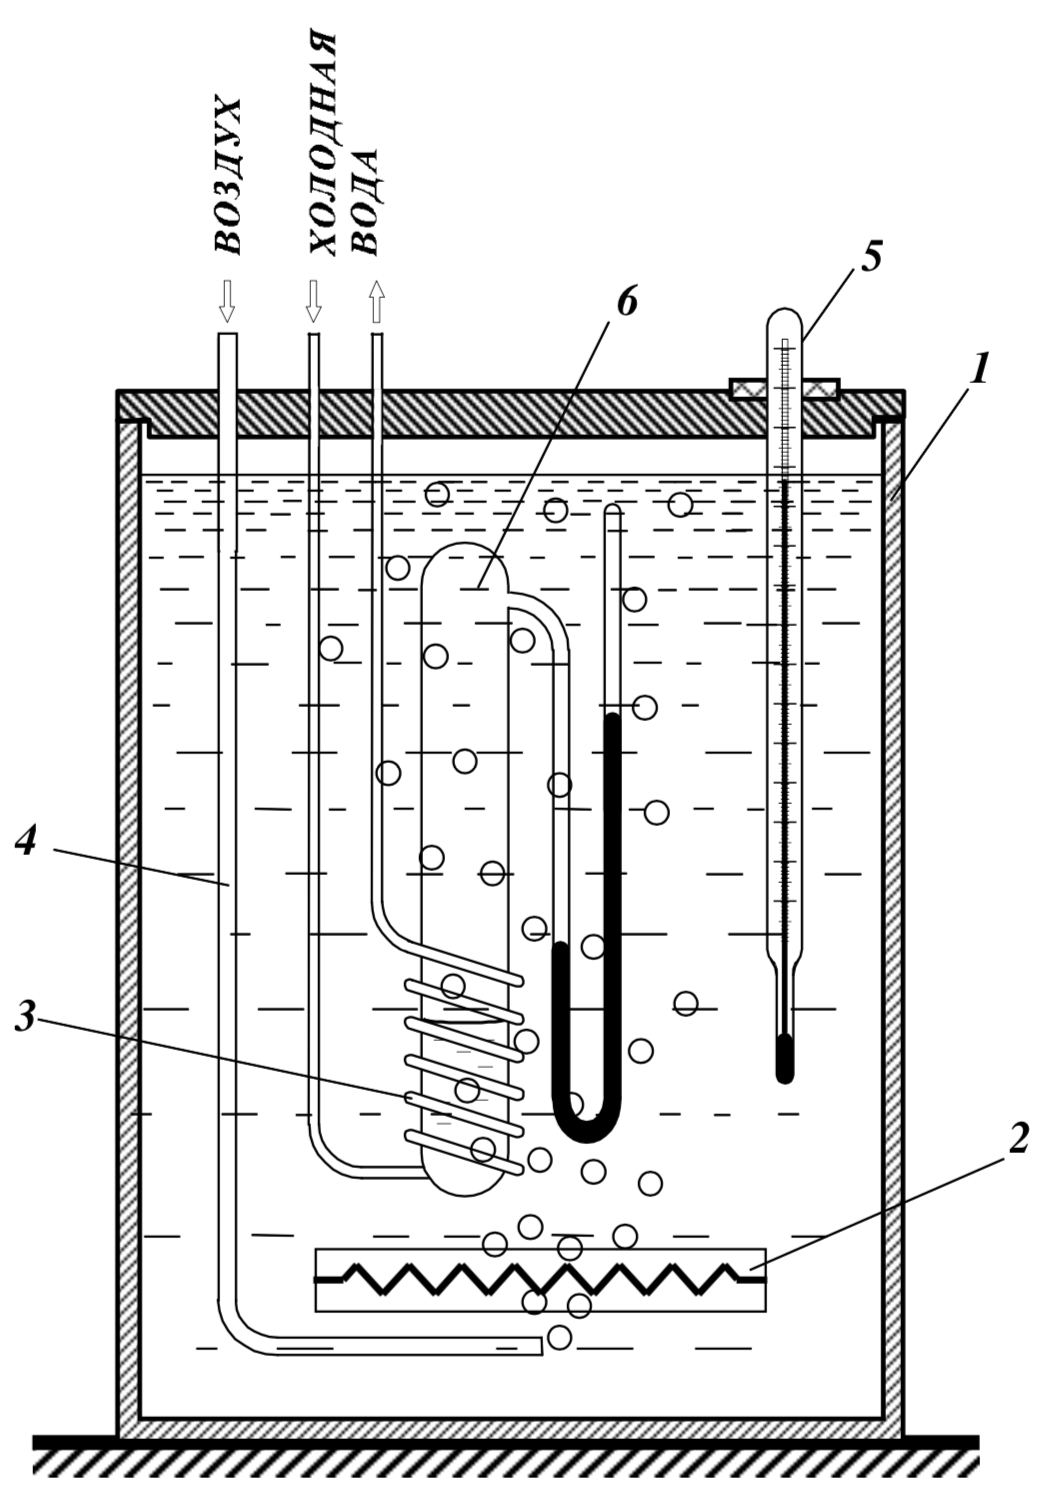
\includegraphics[width=\linewidth]{1}
	\captionsetup{justification=centering}
	\caption{Схема установки для определения теплоты испарения}
\end{wrapfigure}
В работе используются: термостат, герметический сосуд, заполненный исследуемой жидкостью; отсчетный микроскоп
\subsection{Экспериментальная установка}
\noindent Схема установки изображена на рис. 1. 
\begin{enumerate}[label=\arabic* --]
\item Резервуар, наполненный водой, который играет роль термостата
\item  Спираль, нагревающая термостат
\item Змеевик, по которому течет водопроводная вода, которая охлаждает воду в термостате
\item Трубка, через которую поступает воздух, который перемешивается с водой
\item Термометр
\item Запаянный прибор с исследуемой жидкостью, погруженный в термостат
\end{enumerate}
На рис. 2. приведена более полная схема установки.
\begin{figure}[H]
	\begin{center}
	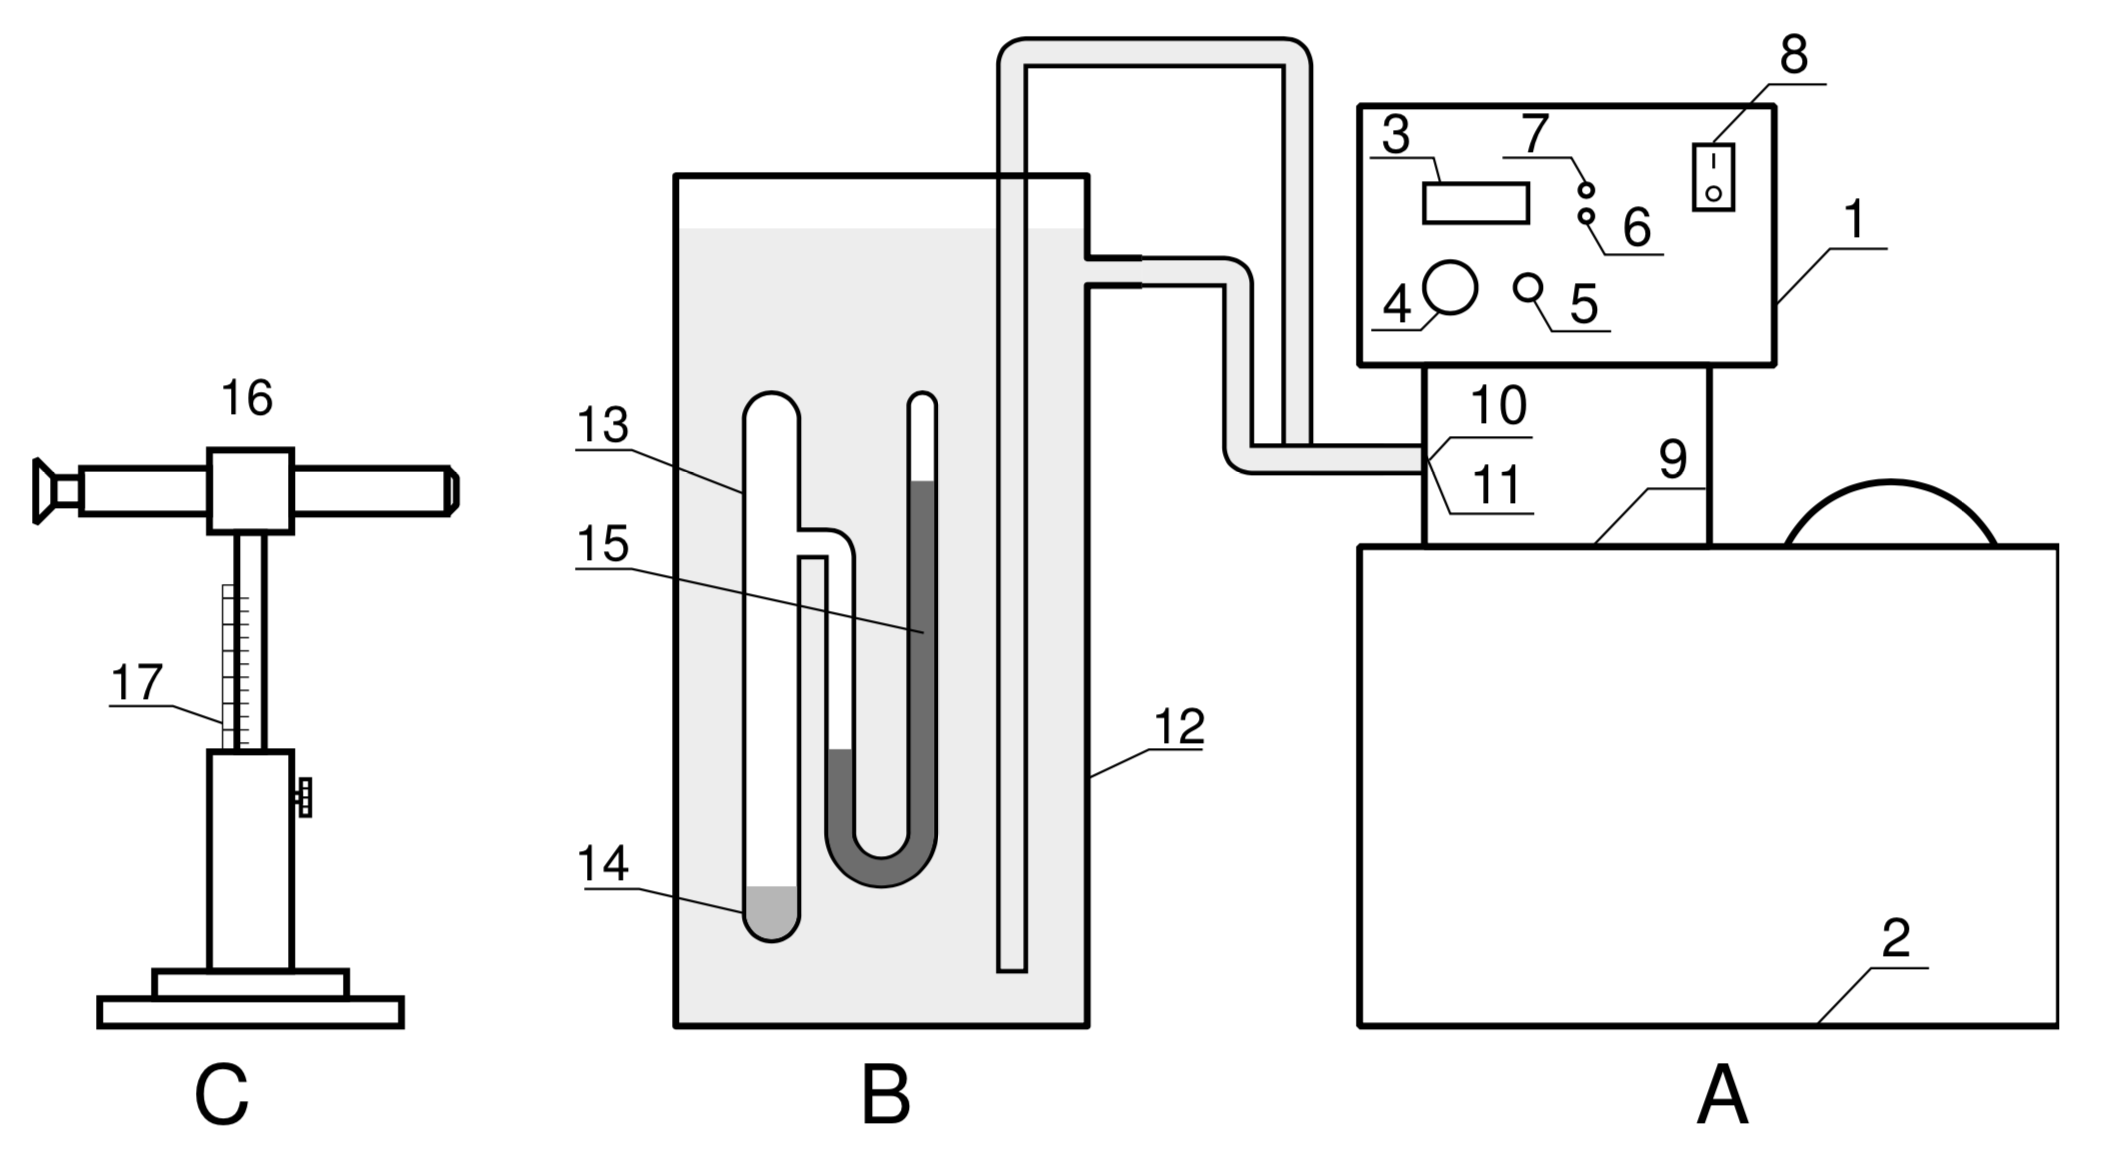
\includegraphics[width=0.7\linewidth]{2}
	\captionsetup{justification=centering}
	\caption{Схема установки для определения теплоты испарения}
	\end{center}
\end{figure}
\noindent Установка включает:
\newcounter{label}
\setcounter{label}{12}
\begin{enumerate}[label=\Alph* --]
	\item Термостат
	\item Экспериментальный прибор
	\begin{enumerate}[label=\arabic{label} --]
		\item Емкость, заполненная водой
		\addtocounter{label}{1}
		\item Запаянный прибор c исследуемой жидкостью
		\addtocounter{label}{1}
		\item Исследуемая жидкость
		\addtocounter{label}{1}
		\item Ртутный манометр
		\addtocounter{label}{1}
	\end{enumerate}
	\item Отсчетный микроскоп
	\begin{enumerate}[label=\arabic{label} --]
		\item Микроскоп, настраиваемый последовательно на нижний\\ и верхний уровни столбика ртути манометра
		\addtocounter{label}{1}
		\item Шкала, по которой снимаются показания
	\end{enumerate}
\end{enumerate}
\subsection{Преимущества и недостатки и  метода измерения}
	Описание прибора указывает на существенное преимущество предложенного косвенного метода измерения $L$ перед прямым. При непосредственном измерении теплоты испарения опыты нужно производить при неизменном давлении, и прибор не может быть запаян. При этом невозможно обеспечить такую чистоту и неизменность экспериментальных условий, как при нашей постановке опыта.
	
	Описываемый прибор обладает важным недостатком: термометр определяет температуру термостата, а не исследуемой жидкости (или
ее пара). Эти температуры близки друг к другу лишь в том случае, если нагревание происходит достаточно медленно.
	\section{Результаты измерений и обработка результатов}

	\renewcommand{\arraystretch}{1} %% increase table row spacing
	\renewcommand{\tabcolsep}{2ex}   %% increase table column spacing
	\begin{table}[H]
		\begin{center}
		\begin{tabular}{|c|c|c||c|c|c|}
			\hline
			\multicolumn{3}{|c||}{Нагревание}  & \multicolumn{3}{|c|}{Охлаждение}     \\ \hline
			$T, \text{К}$      & $p, \text{Па}$      & $\Delta p, \text{Па}$      & $T, \text{К}$      & $p, \text{Па}$      & $\Delta p, \text{Па}$     \\ \hline
			297,92 & 2958,8 & 133,37 & 311,42 & 4454,9 & 87,87 \\ \hline
			298,77 & 3038,8 & 133,38 & 310,60 & 4215,0 & 86,20 \\ \hline
			299,82 & 3252,0 & 133,39 & 309,65 & 4081,7 & 85,21 \\ \hline
			300,93 & 3452,0 & 133,40 & 308,81 & 3695,2 & 82,12 \\ \hline
			301,93 & 3611,9 & 133,41 & 307,50 & 3375,3 & 79,23 \\ \hline
			302,95 & 3838,5 & 133,43 & 306,56 & 3082,1 & 76,29 \\ \hline
			304,01 & 4118,4 & 133,45 & 305,51 & 2775,6 & 72,85 \\ \hline
			304,97 & 4318,3 & 133,47 & 304,50 & 2535,7 & 69,85 \\ \hline
			305,95 & 4544,8 & 133,49 & 303,64 & 2295,7 & 66,54 \\ \hline
			307,05 & 4891,4 & 133,52 & 302,67 & 2055,8 & 62,87 \\ \hline
			308,91 & 5331,2 & 133,56 & 301,70 & 1842,6 & 59,25 \\ \hline
			309,98 & 5651,1 & 133,59 & 300,57 & 1736,0 & 57,29 \\ \hline
			311,05 & 6117,6 & 133,64 & 299,57 & 1442,8 & 51,34 \\ \hline
			312,05 & 6384,1 & 133,67 & 298,60 & 1229,5 & 46,40 \\ \hline
			313,05 & 6757,3 & 133,72 & 297,65 & 1109,6 & 43,34 \\ \hline
		\end{tabular}
	\captionsetup{justification=centering}
	\caption{Зависимость давления $p$ от температуры $T$ при нагревании и охлаждении}
	\end{center}
	\end{table}
	\renewcommand{\tabcolsep}{1.5ex}
\begin{table}[H]
	\begin{center}
	\begin{tabular}{|c|c|c||c|c|c|}
		\hline
		\multicolumn{3}{|c||}{Нагревание}  & \multicolumn{3}{|c|}{Охлаждение}     \\ \hline
		\rule{0cm}{2.5ex}
		$1/T, \text{К}^{-1}$      & $\ln p, \text{Па}$      & $\Delta \ln p,$      & $1/T, \text{К}^{-1}$      & $\ln p, \text{Па}$      & $\Delta \ln p,$     \\\hline
		3,36 & 7,99 & 0,36 & 3,21 & 8,81 & 0,17 \\ \hline
		3,35 & 8,02 & 0,35 & 3,22 & 8,77 & 0,17 \\ \hline
		3,34 & 8,09 & 0,33 & 3,23 & 8,75 & 0,17 \\ \hline
		3,32 & 8,15 & 0,31 & 3,24 & 8,69 & 0,18 \\ \hline
		3,31 & 8,19 & 0,30 & 3,25 & 8,64 & 0,19 \\ \hline
		3,30 & 8,25 & 0,29 & 3,26 & 8,58 & 0,20 \\ \hline
		3,29 & 8,32 & 0,27 & 3,27 & 8,52 & 0,21 \\ \hline
		3,28 & 8,37 & 0,26 & 3,28 & 8,48 & 0,22 \\ \hline
		3,27 & 8,42 & 0,25 & 3,29 & 8,42 & 0,22 \\ \hline
		3,26 & 8,50 & 0,23 & 3,30 & 8,37 & 0,23 \\ \hline
		3,24 & 8,58 & 0,21 & 3,31 & 8,32& 0,24 \\ \hline
		3,23 & 8,64 & 0,20 & 3,33 & 8,29 & 0,25 \\ \hline
		3,21 & 8,72 & 0,19 & 3,34 & 8,22 & 0,26 \\ \hline
		3,20 & 8,76 & 0,18 & 3,35 & 8,16 & 0,27 \\ \hline
		3,19 & 8,82 & 0,17 & 3,36 & 8,13 & 0,27 \\ \hline
	\end{tabular}
\captionsetup{justification=centering}
\caption{Зависимость логорифма давления $\ln p$ от величины, обратной к температуре $1/T$ при нагревании и охлаждении}
\end{center}
\end{table}
Cнимем Зависимость давления $p$ от температуры $T$ при нагревании и охлаждении. Результаты занесем в Таблицу 2. Перепишем Таблицу 2, переходя к $\ln p$ и $1/T$.

По данным таблицы 2 и 3 построим графики зависимости давления от температуры при нагревании и охлаждении.

\begin{figure}[H]
	\begin{center}
	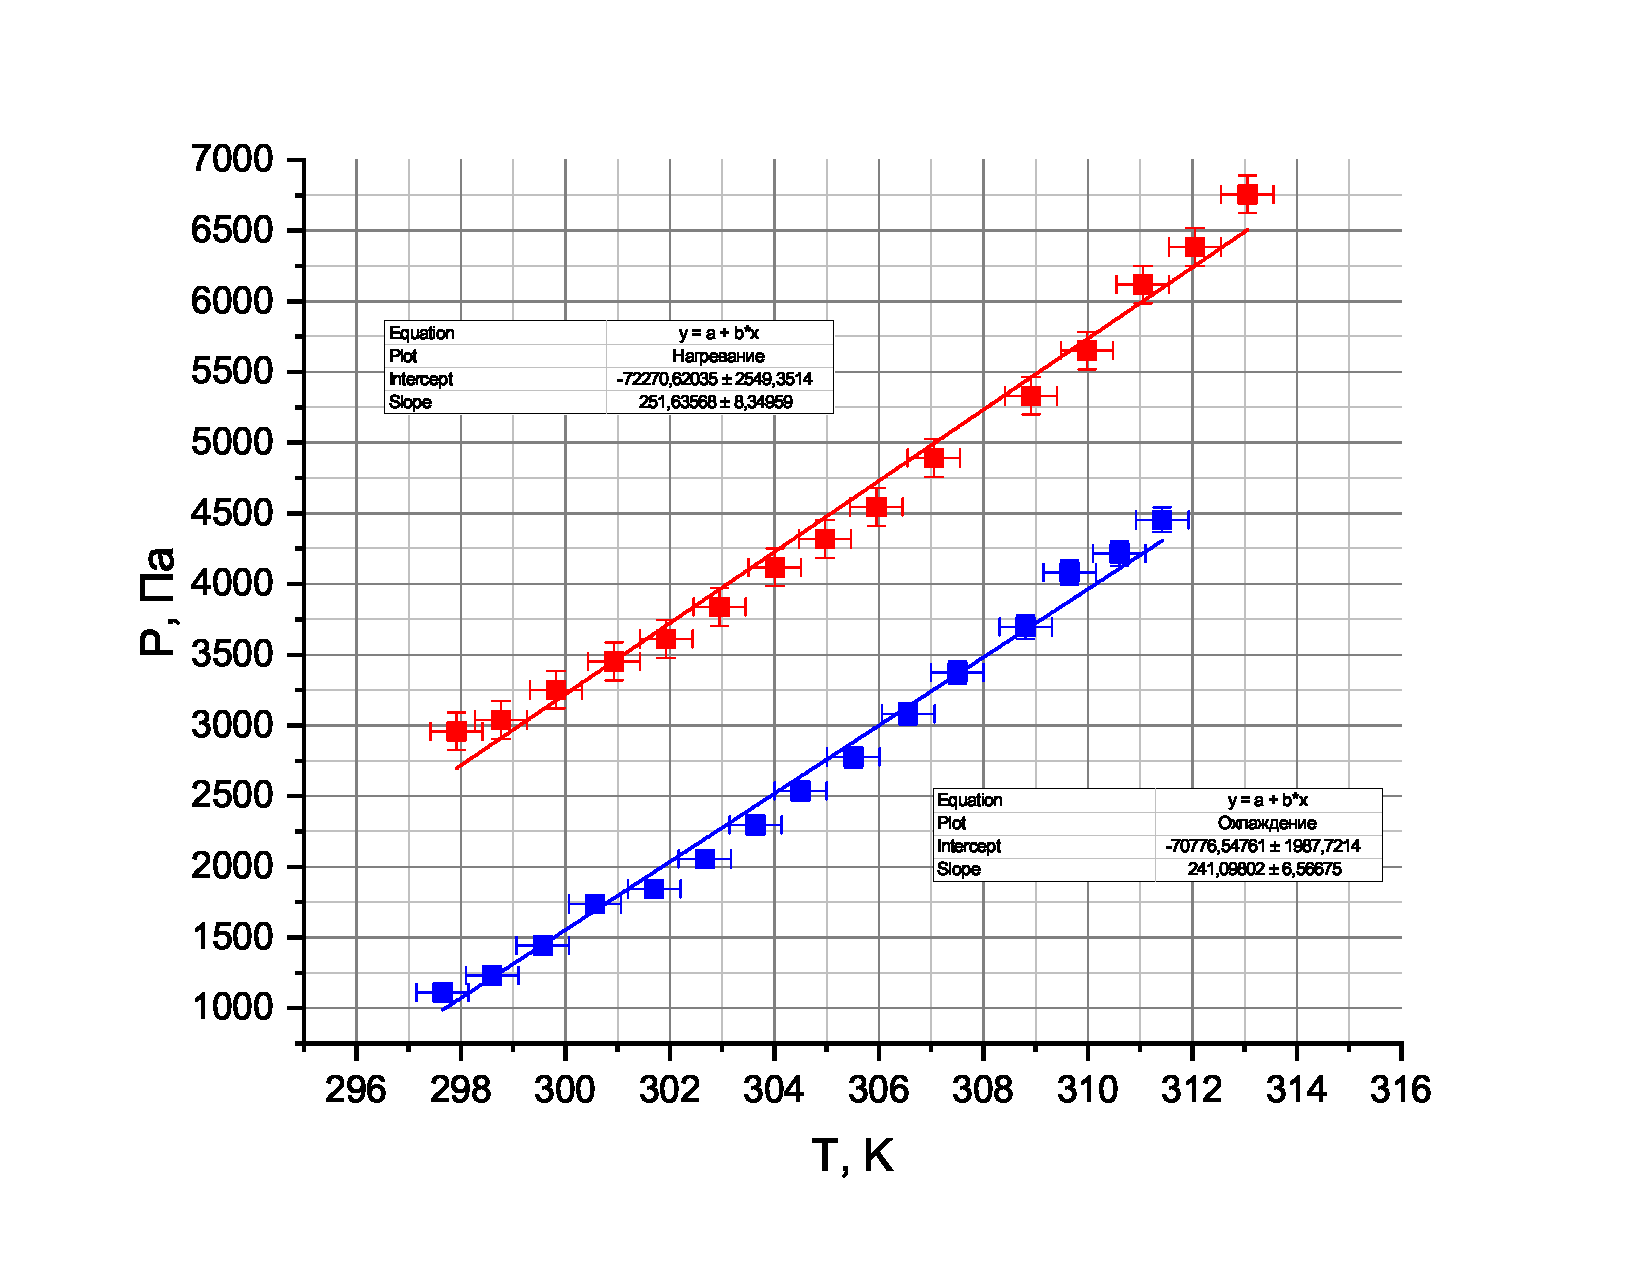
\includegraphics[width=\linewidth]{3}
	\captionsetup{justification=centering}
	\caption{Зависимость давления $p$ от температуры $T$ при нагревании и охлаждении}
\end{center}
\end{figure}
Используя формулу (4) рассчитаем теплоту испарения воды по рис. 4:
\[L_\text{+} = (43,2\pm 0,4)\text{КДж}/\text{моль}\]
\[L_\text{-} = (39,2\pm 0,5)\text{КДж}/\text{моль}\]
\begin{figure}[H]
	\begin{center}
		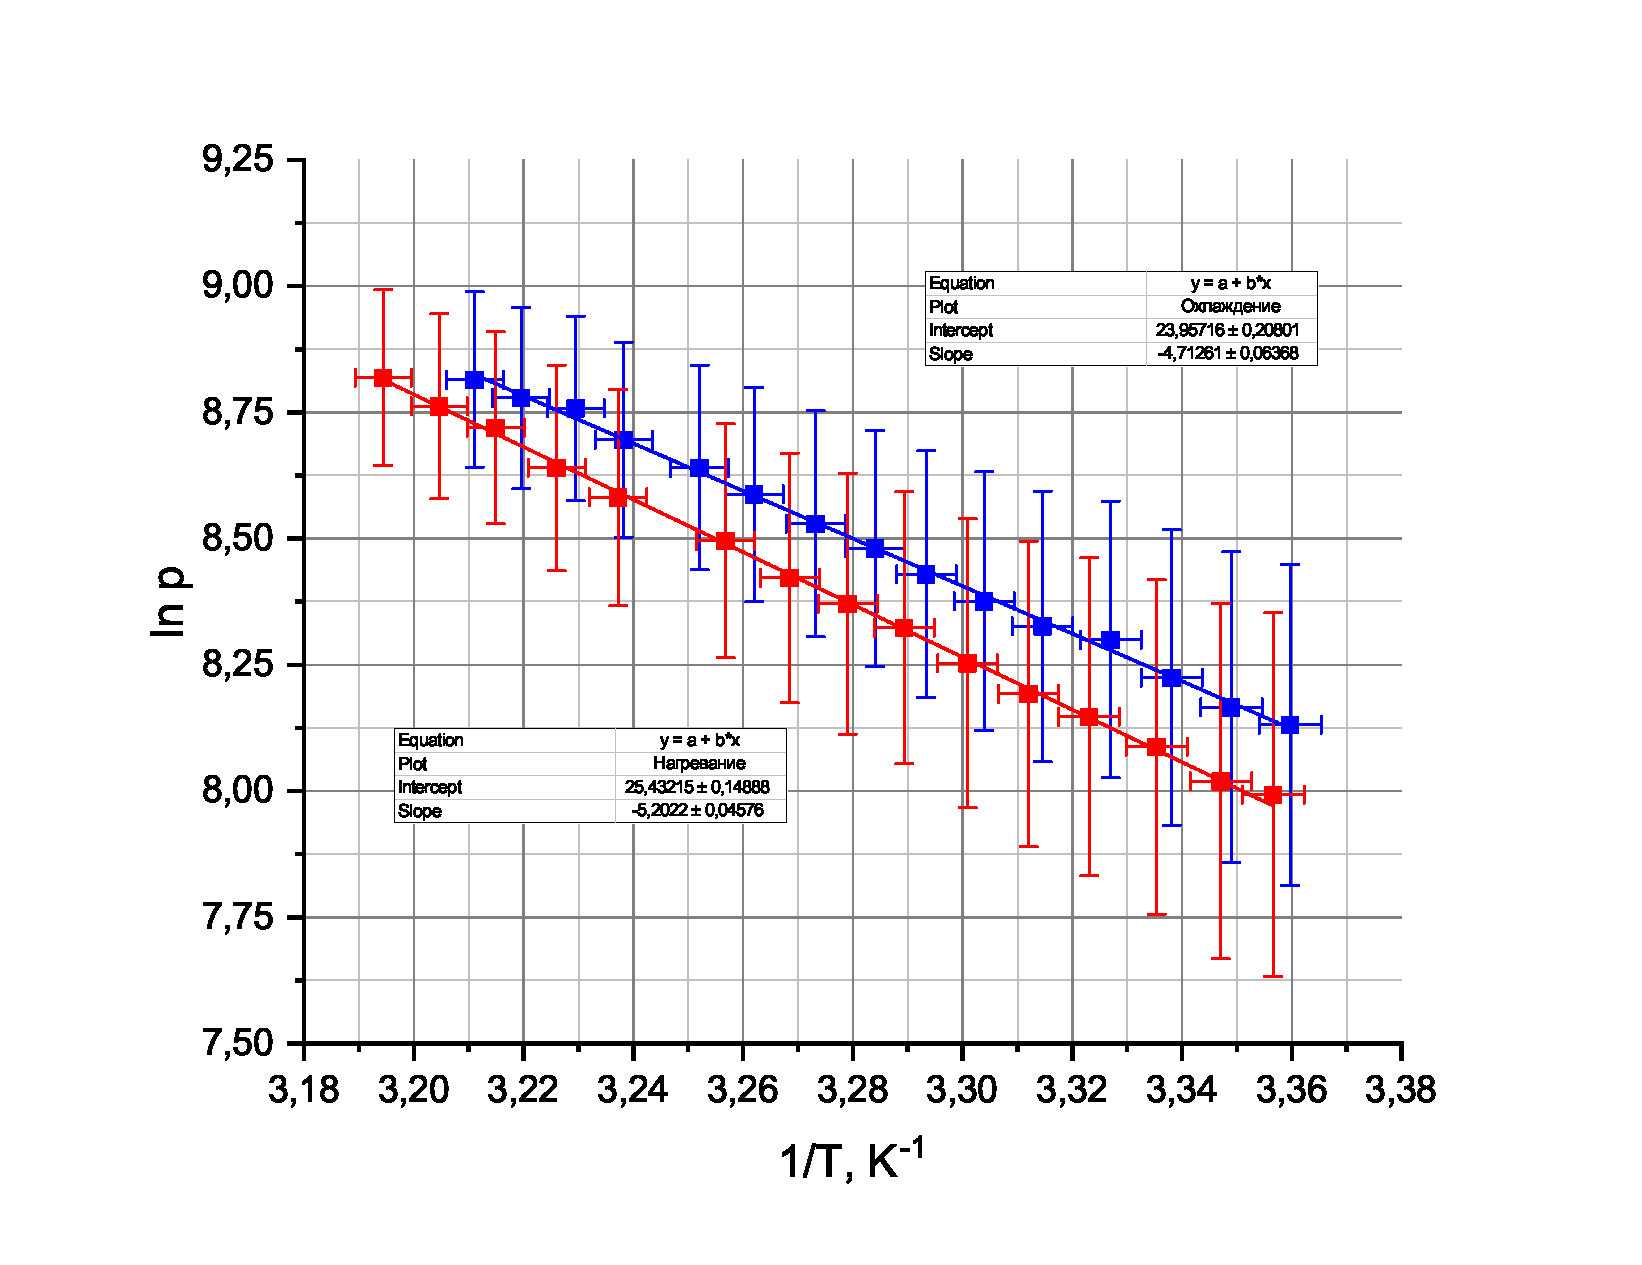
\includegraphics[width=\linewidth]{4}
		\captionsetup{justification=centering}
		\caption{Зависимость логорифма давления $\ln p$ от величины, обратной к температуре $1/T$ при нагревании и охлаждении}
	\end{center}
\end{figure}
\section{Обсуждение результатов и выводы}
В работе были получены значения для теплоты испарения воды при нагревании и охлаждении:
\[L_\text{+} = (43,2\pm 0,4)\text{КДж}/\text{моль}\]
\[L_\text{-} = (39,2\pm 0,5)\text{КДж}/\text{моль}\]
\[L = (41,2\pm 0,6)\text{КДж}/\text{моль}\]
Значения удовлетворяют табличным. При этом значения $L_\text{+}$ и $L_\text{-}$ будут совпадать при небольшом изменении точек для апроксимации. Это очень хорошо видно из Рис. 4. Что полностью соотносится с теоритическими выводами.
\end{document}